% --------------------------------------
%       PLEASE SEE README.MD
% --------------------------------------

\documentclass[
    letterpaper,
    10pt,
    unnumberedsections,
    twoside
]{LTJournalArticle}

\runninghead{Biomimetic Hydrogel-Scaffold for Tendon and Ligament Repair}
\footertext{}

\usepackage{lipsum} % Lorem ipsum text for formatting
\usepackage{chemfig}
\usepackage{dblfloatfix}

\addbibresource{references_lucas.bib}
\addbibresource{references_edison.bib}

\title{Biomimetic Hydrogel-Scaffold for Tendon and Ligament Repair}
\author{Lucas Chan, Luke Gailloux, Matt Levasseur, Edison Luke}

\renewcommand{\maketitlehookd}{%
    \begin{abstract}
        \noindent \lipsum[1]
    \end{abstract}
}

\setlength{\parskip}{0pt plus 1pt}

\begin{document}
    \maketitle 

    \section{Introduction}

    Sample introduction for formatting testing.

\lipsum[1]

    \section{Hydrogel Structure and Composition}

    Hydrogels are 3D crosslinked polymer structures containing hydrohpilic functional groups, allowing them to absorb large quantities of water. Because of this, they are flexible and soft, and resemble many natural tissues \autocite{hoHydrogelsPropertiesApplications2022}.
Recent advances in hydrogel technology have led to the development of implantable and injectable hydrogels with potential applications in drug delivery. By adjusting polymer composition, key properties such as swelling-deswelling rate, stiffness, and degradability can be fine-tuned to meet specific use case requirements. As biomedical applications of hydrogels continue to expand, their use in tendon and ligament repair presents a promising opportunity.

Hydrogel cross-linked chains can be formed using natural, synthetic, or semi-synthetic polymers. Natural polymers such as cellulose, chitosan, and collagen are inherently biocompatible and bioactive, but come at the cost of weak stability and poor mechanical strength. Being derived from natural sources, these hydrogels are generally safe to use in clinical applications, but have shown to be allergens in rare cases \autocite{hoHydrogelsPropertiesApplications2022}.

On the other hand, synthetic hydrogels are made of man-made polymers like polyvinyl alcohol (PVA), polyethylene glycol (PVG), or polyacrylamide (PAAM). Few of these synthetic materials have been shown to be biocompatible, but they offer superior mechanical strength and stability \autocite{hoHydrogelsPropertiesApplications2022}.

To achieve both the biocompatibility offered by natural hydrogels and the strength and mechanical properties offered by their synthetic counterparts, a common approach is to develop a hybrid, or semi-synthetic hydrogel chain. Hybrid hydrogels can either be made by chemically modifying natural polymers or by blending natural and synthetic components.

    \section{Self-Healing ``Smart'' Hydrogels}
    When subjected to physical or chemical stimuli, ``smart'' hydrogels have the ability to dynamically modify their physical properties, such as mechanical strength and swellability \autocite{hoHydrogelsPropertiesApplications2022}.
Self-healing hydrogels are a subset of smart hydrogels. These hydrogels are made of dynamic cross-linkages that can spontaneously re-form after having sustained mechanical damage. Self-healing properties allow the hydrogel to have superior mechanical toughness and a longer life span \autocite{deviv.k.SelfHealingHydrogelsPreparation2021}.

Self-healing hydrogels are unique in that the polymer chains are bound together by dynamic cross-linkages that can spontaneously self-repair. These cross-linkages can be the result of covalent or non-covalent interactions.
Covalent cross-linkages include imine and disulfide bonds. They are higher in energy and are therefore more difficult to break. Because of this, they are generally more stable and have superior mechanical strength.
Reversible non-covalent dynamic linkages arise from interactions such as hydrogen bonding, ionic interactions, and hydrophobic effects. These bonds are easily broken and reconstructed, which leads to a more flexible but mechanically weaker hydrogel \autocite{deviv.k.SelfHealingHydrogelsPreparation2021}.

\subsection{Self-Healing by Imine Bonds}

Imine bonds for self-healing hydrogels show promise in biomedical applications, especially in wound healing and in tissue engineering. Imines are chemical compounds containing a carbon atom doubly-bonded to a nitrogen. They are stabilised when the nitrogen atom contains an aromatic ring as a substituent, in which case it is known as a Schiff base \autocite{moldoveanuChapter8Pyrolysis2019}.
The C=N imine bond is formed when an aldehyde reacts with an amine, forming the Schiff base. This reaction is reversible, meaning that the imine bond can break and reform spontaneously given the appropriate conditions.

\begin{figure}[ht]
    \setchemfig{atom sep=2em}
    \centering
    \chemfig{
        *6((-R_1)=-=(-=[::-60]N-R_2)-=-)
    }
    \caption{Bond-line illustration of a Schiff base}
    \label{fig:schiff_base}
\end{figure}

    \section{Mechanical Properties of Janus Tough Adhesive Hydrogels}

    In addition to biocompatibility, the mechanical properties of a given hydrogel decide whether or not a given hydrogel is functional. In particular, hydrogels must have sufficient toughness and adhesive strength \autocite{Freedman.EnhancedTendonHealing}. In vivo, tendons must withstand a dynamic environment and bear strong forces \autocite{Chen.AdvancesApplicationHydrogel}; thus, a hydrogel must be able to withstand sufficient amounts of force without fracturing – that is, an ideal hydrogel should only deform plastically (Freedman et al.). Furthermore, to promote optimal healing, hydrogels should be placed and remain near the relevant tendon. However, force generated by movement can lead to hydrogel displacement; Hence, adhesion is required to ensure immobility (Freedman et al.). A variety of strategies can be implemented on a biochemical level to greatly increase the toughness and adhesiveness in order to create an adequate hydrogel for tendon repair.

This is still a test
High mechanical toughness of the JTA was achieved using a dual interpenetrating hydrogel network that combines the ability of alginate hydrogels to dissipate energy through dissociation of ionic bonds with a highly elastic covalently cross-linked acrylamide hydrogel that can distribute stresses throughout the network. \cite{FreedmanEnhancedTendonHealing}

The backbone structure of the tough SL was polyacrylic acid (PAA) networks, with long-chain glycidyl methacrylate-modified chondroitin sulfate (CSMA) as the cross-linking agent and encapsulated chondroitin sulfate (CS), which endowed the JHA with strong mechanical properties for effectively dissipating energy under deformation \cite{JuSurfaceEnzymePolymerization}

The interlocking structure and continuous features of the JHA were also confirmed from the Raman mapping image in Fig. 2i. This interlocked structure firmly bonded the two layers, and the RL could effectively transfer the strain to the SL through the interlocking structure, avoiding fracture and delamination, thereby achieving stable and robust adhesion to biological tissues. \cite{JuSurfaceEnzymePolymerization}



    \section{Biocompatibility}

    The Janus Tough Adhesive has shown to exhibit high biocompatibility during testing, despite it containing the synthetic polymer polyacrylamide. To evaluate their performance and impact on natural tissues, \citeauthor{freedmanEnhancedTendonHealing2022} (\citeyear{freedmanEnhancedTendonHealing2022}) experimentally tested  injured and healthy rats, and applied the JTA to the patellar tendon.
For three weeks, potential swelling of the tendon and degredation of the gel were assessed by high frequency ultrasound. When a tendon becomes injured, its echogenicity---the amount of sound it reflects---decreases, because its collagen fibres become more disorganised and less densely packed \autocite{hodgsonTendonLigamentImaging2012}.
Researchers also found that injured tendons without application of the JTA had larger cross-section areas, indicating increased swelling as shown in Figure~\ref{fig:JTA_Patellar_cross_section}. A decrease in inflammation in the affected tendon therefore suggests that the JTA was effective and well-tolerated by the body.
\begin{figure*}[ht]
    \centering
    \begin{minipage}[b]{0.45\textwidth}
        \centering
        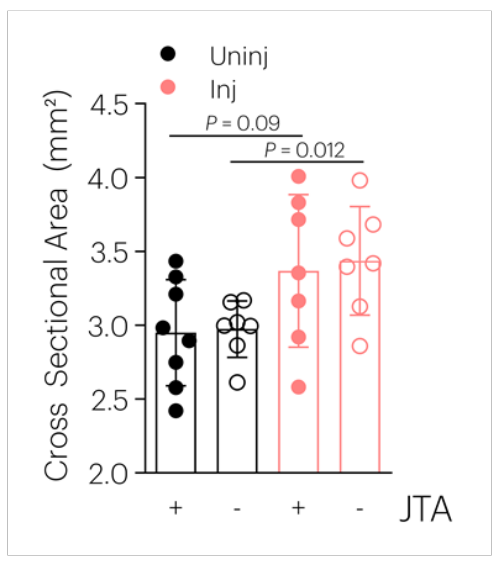
\includegraphics[width=0.6\linewidth]{JTA_cross_section.png}
        \caption{Patellar tendon cross-sectional area (mm\textsuperscript{2}) after 3 weeks of treatment [Adapted from \cite{freedmanEnhancedTendonHealing2022}]}
        \label{fig:JTA_Patellar_cross_section}
    \end{minipage}
    \hfill
    \begin{minipage}[b]{0.45\textwidth}
        \centering
        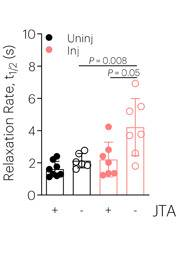
\includegraphics[width=0.6\linewidth]{Figures/JTA_relaxation_patellar.jpeg}
        \caption{Patellar tendon relaxation rate [Adapted from \cite{freedmanEnhancedTendonHealing2022}]}
        \label{fig:JTA_Patellar_relaxation}
    \end{minipage}
\end{figure*}

Furthermore, in the patellar tendon, the JTA was found to have improved tendon relaxation (Figure~\ref{fig:JTA_Patellar_relaxation}), without impacting natural properties such as elastic mechanics, dynamic modulus, or linear modulus.

% Biocompatibility of the JTA was also tested in more complex use cases, such as the rotator cuff and Achilles tendon. 

    \section{Towards a Self-Healing JTA}

    \begin{figure*}[hb]
    \centering 
    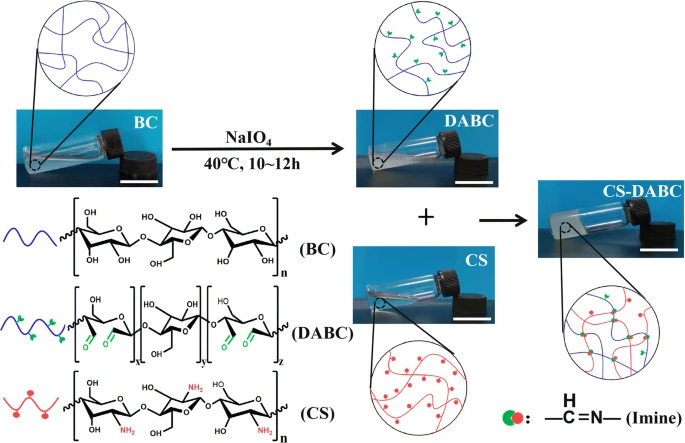
\includegraphics[width=0.7\linewidth]{Figures/CS_DABC_condensation.jpg}
    \caption{Schematic representation of hydrogel synthesis from chitosan and dialdehyde bacterial cellulose \autocite{liAllnaturalInjectableHydrogel2020}}
    \label{fig:CS_DABC_condensation}
\end{figure*}

\section{Towards a Self-Healing JTA}

A recent study by \citeauthor{liAllnaturalInjectableHydrogel2020} found that an all-natural, injectable hydrogel could be synthesized using chitosan and dialdehyde bacterial cellulose (\citeyear{liAllnaturalInjectableHydrogel2020}). This hydrogel uses imine bond dynamic cross-linkages to achieve its self-healing properties, where the Schiff base forms through the reaction of chitosan (as the amine) and bacterial cellulose (as the aldehyde).
The reaction can proceed under mild conditions (room temperature and pH = 7.2), and as it is all-natural, it has shown to be biocompatible. A schematic representation of this condensation reaction is given in Figure~\ref{fig:CS_DABC_condensation}.

Researchers tested the CS-DABC hydrogel's ability to self-repair after sustaining damage, a property that is desired for applications in wound dressings. To do so, round hydrogels were prepared and cut in half. One side was coloured orange, and the two half-discs were placed side-by-side in ambient conditions, as shown in Figure~\ref{fig:CS_DABC_self_healing}.
In just 3 hours, without external intervention, the two halves fused back together and reformed the original shape. They were also able to be picked up by one side, withstanding the force of gravity. Moreover, the gaps between the two hydrogel half-discs were observed under optical microscope.
The boundaries between the two sides were barely visible, demonstrating good self-healing properties from Schiff base reactions.

\begin{figure}[ht]
    \centering 
    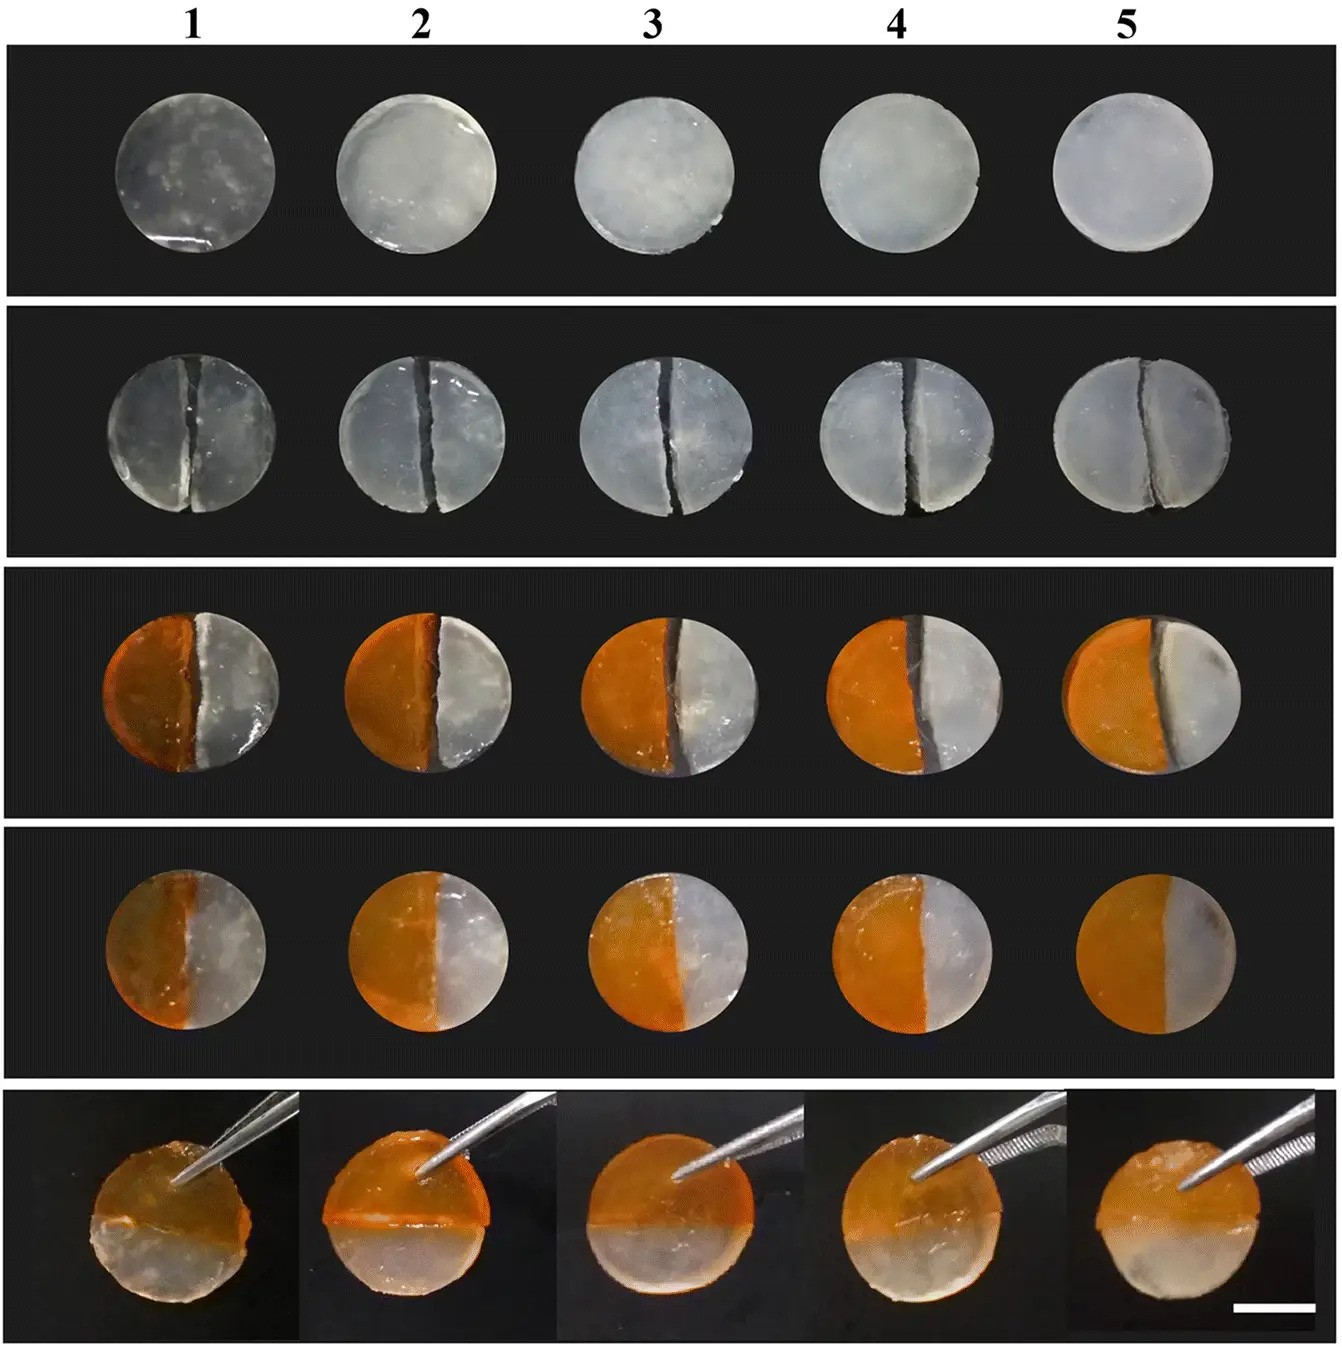
\includegraphics[width=\linewidth]{Figures/CS_DABC_self_healing.jpg}
    \caption{Self-healing properties of CS-DABC hydrogels. Discs were cut, stained, and healed under ambient conditions. [Adapted from \cite{liAllnaturalInjectableHydrogel2020}]}
    \label{fig:CS_DABC_self_healing}
\end{figure}

Additionally, the chitosan dressing exhibits antimicrobial properties, which reduces the risk of cross-contamination and promotes healthy healing of the wound. To evaluate these properties, the hydrogel was tested as an antibiotic against strains of \textit{E. coli} and \textit{S. aureus}.
Far fewer bacterial colonies were observed in the samples treated with CS-DABC compared to the control. As the hydrogel's protonated amino groups bind to the bacterial cell wall, effectively destroying it, bacterial growth is inhibited \autocite{liAllnaturalInjectableHydrogel2020}.

This self-healing hydrogel presents a promising application for tendon repair. Since JTAs already have a chitosan layer, it could be possible to synthesize Schiff bases directly on the existing structure using a similar technique as \citeauthor{liAllnaturalInjectableHydrogel2020}, leading to increased mechanical strength through the integration of self-healing properties.
% This self-healing hydrogel, therefore, has an interesting application for tendon repair. Given that JTAs have a chitosan side, it could be possible to augment their mechanical strength by integrating self-healing properties.
\end{document}